Raft mode provides a less performant yet more reliable replication scheme for Pub/Sub. In master-slave mode

\begin{figure}[H]
	\centering
	\begin{tikzpicture}[shorten >=1pt,node distance=2cm,on grid,auto]
		\node[state] (0) {peer-0};
		\node[state] (1) [right=of 0]{peer-1};
		\node[state] (2) [below=of 0]{peer-2};
		\node[state] (3) [right=of 2]{peer-3};
		\path[->]
			(0) edge node {} (1)
			(0) edge node {} (2)
			(0) edge node {} (3)
			
			(1) edge node {} (0)
			(1) edge node {} (2)
			(1) edge node {} (3)
			
			
			(2) edge node {} (0)
			(2) edge node {} (1)
			(2) edge node {} (3)
			
			
			(3) edge node {} (0)
			(3) edge node {} (1)
			(3) edge node {} (2);
	\end{tikzpicture}
	\caption{Raft Cluster Topology}
\end{figure}
	
\begin{figure}[H]
	\centering
	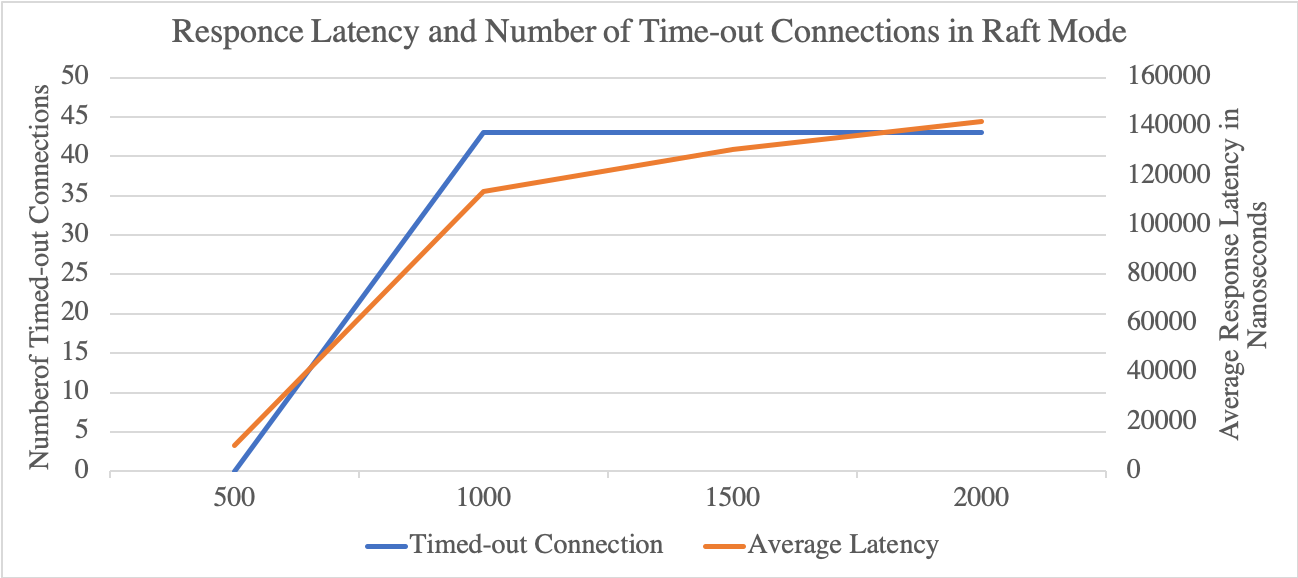
\includegraphics[scale=0.33]{figure/raft/performance.png}
	\caption{Raft Performance}
\end{figure}
	
\begin{figure}[H]
	\centering
	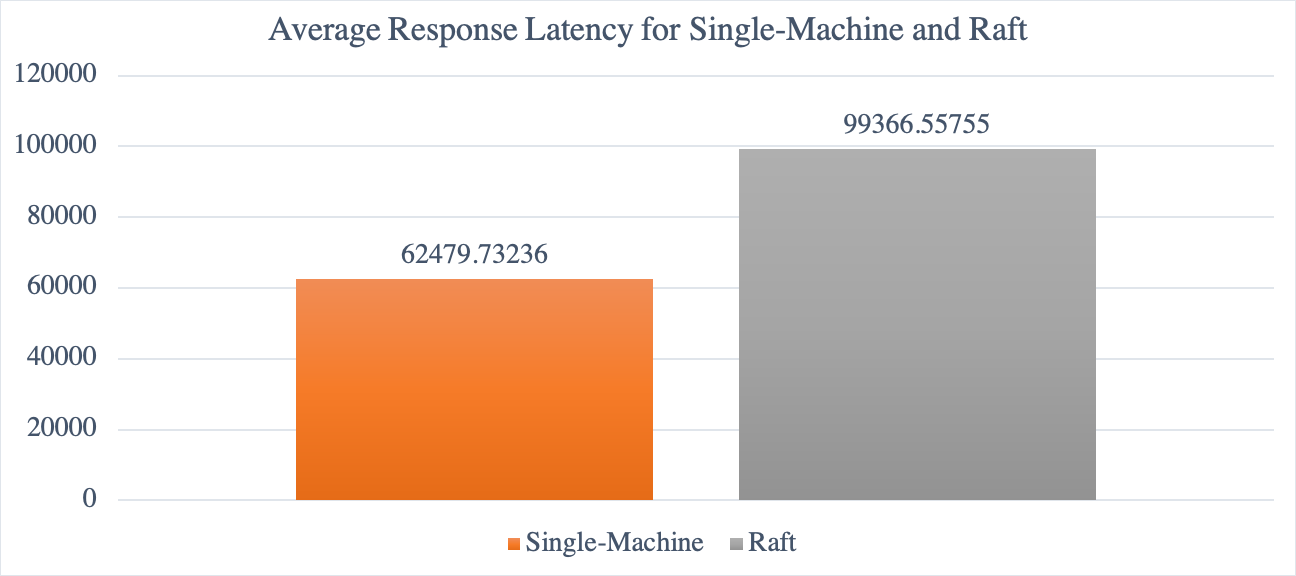
\includegraphics[scale=0.33]{figure/raft/response-latency.png}
	\caption{Single-Machine/Raft average response latency}
\end{figure}

% TODO (zcdirk@)
% Talk about optimization strategies in Raft implementation
